\section{Navegação} % (fold)
\label{sec:navegação2}
	
	Como o processamento de todas as informações obtidas durante a navegação ocorrerá na base, sabe-se que o tempo de resposta do servidor é uma variável importante quando se refere a um sistema de tempo real, como o proposto pelo projeto. Dessa maneira, fez-se necessária a implantação do \textit{patch} \textit{rt\_preempt} no kernel do linux presente na \textit{raspberry}. Para isso, utilizamos como fonte de conhecimento a wiki oficial do projeto \textit{RT\_preempt}, disponível \href{https://rt.wiki.kernel.org/index.php/Main_Page}{aqui}.

	Com a configuração e recompilação do kernel com este \textit{patch}, obtivemos um tempo de resposta aproximado de 19 micro segundos, o que foi considerado bom pela equipe do projeto. Uma análise foi feita utilizando o \textit{script} \textit{cylicltest}, da mesma equipe \textit{RT\_preempt}, para calcular o tempo mínimo, médio e máximo de resposta. Na simulação foi utilizado um processo com prioridade 80, com 100.000 (cem mil) \textit{loops} a um intervalo de 500 micro segundos, obtendo o resultado apresentado na Figura \ref{img:tempo_de_resposta}.

	\begin{figure}[H]
		\centering
		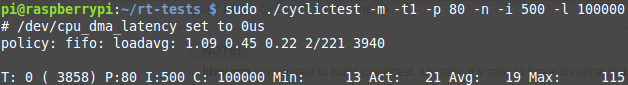
\includegraphics[scale=0.7]{figuras/tempo_de_resposta.png}
		\caption{Tempo de resposta do servidor.}
		\label{img:tempo_de_resposta}
	\end{figure}

	Após a implantação deste requisito de tempo real, buscou-se definir uma estratégia de navegação que contemple os requisitos iniciais do projeto. Para isso, o sistema de navegação foi dividido em 2 contextos. A navegação pode estar no contexto de \textit{running}, onde estará rodando pelo ambiente de maneira aleatória, ou \textit{back}, no qual o robô deverá retornar para base.

	Nos sub-tópicos a seguir estão detalhadas as estratégias de navegação nos dois contextos.

	\subsection{Running} % (fold)
	 \label{sub:running}
	 
	 	O algoritmo de navegação utilizado durante este contexto é bastante simples, o qual envolve uma estratégia de navegação aleatória. Basicamente, o robô sempre tenderá a andar para frente, quando for encontrado um obstáculo, o servidor enviará uma ordem para desviar daquele obstáculo, levando em consideração as distâncias laterais do robô. Para isso, o robô utiliza 4 sonares, um apontado para a frente, e os outros dois apontados um para cada lado do robô.

	 	Esta navegação aletarória ocorre até que seja determinado o recuo à base, seja por falta de bateria ou por entrada \textit{stop} por parte do usuário.

	 	% A utilização de \textit{encoders} é necessária para minimizar a margem de erro na angulação de curvas e distâncias percorridas. Porém, sua utilização está suspensa durante esta segunda fase do projeto, sendo implementado apenas na terceira etapa, fase de integração dos subsistemas.
	 % subsection running (end) 

	 \subsection{De volta à base (Back)} % (fold)
	 \label{sub:de_volta_a_base_}
	 	
	 	O retorno à base deve levar em consideração o tempo disponível de bateria, ou seja, o caminho para base deve ser razoavelmente eficiente. Porém, a utilização da potência de sinal do \textit{wifi} gerou problemas relacionados a precisão destes dados. Por este motivo, o retorno a base também se encontra em estado de implementação. 

	 	De acordo com o apresentado no plano de gerenciamento de risco, disposto no capítulo \ref{cha:riscos}, foi identificado um risco que afeta todo o planejamento incial para retorno a base. Este risco está ligado a precisão dos resultados obtidos com o uso da potência do sinal wifi para retorno a base. A partir de diversos testes, foi observado que a margem de erro deste sinal é muito elevada para utilização em um algoritmo de navegação. Desse modo, sua implementação foi deixada para a terceira etapa do projeto, onde serão utilizados outros meios, seja para calibrar o erro deste sinal, ou para substituir esta estratégia.

	 	Durante esta etapa do trabalho, a estratégia para retorno a base envolve a utilização de um emissor na base, com um receptor no robô identificando a distância do emissor. Com esta informação, é possível navegar pelo ambiente realizando comparações de resultados para traçar uma direção até a base. De acordo com análises experimentais, é possível identificar a direção da base utilizando apenas 3 pontos distintos no ambiente. Estes pontos devem estar separados a uma distância inversamente proporcional a precisão deste sinal analisado.

	 	Visualizando cada distância como um raio de uma circunferência, com 3 pontos obtidos pode-se analisar 3 circunferências que deverão possuir um ponto de intersecção, o qual deverá apontar para a base. Com o objetivo de simplificar a explicação, a Figura \ref{img:back} apresenta uma simulação da estratégia de retorno a base.

	 	\begin{figure}[H]
			\centering
			\includegraphics[scale=0.14]{figuras/volta_a_base.png}
			\caption{Estratégia para identificação da direção da base.}
			\label{img:back}
		\end{figure} 

		É importante ressaltar que para que a estratégia funcione, os 3 pontos não podem ser colineares, pois se forem o resultado das leituras pode acabar gerando dois pontos possíveis de intersecção, como mostrados no exemplo da figura \ref{img:back2}

		\begin{figure}[H]
			\centering
			\includegraphics[scale=1]{figuras/volta_a_base_colinear.png}
			\caption{Estratégia para identificação da direção da base com pontos colineares.}
			\label{img:back2}
		\end{figure} 
	 % subsection de_volta_a_base_ (end)

	 \subsection{Testes}
	
		Ainda não foram realizados testes neste subsistema. Os testes com relação ao running não será realizado pois o robô irá andar de forma aleatória. Com relação ao back, o teste será feito colocando o robô com alguns obstáculos em diferentes disposições e o robô deverá chegar à base sem se perder.
% section navegação (end)

